\chapter{Test and beam time analysis} \label{analysis}

\begin{outline}[enumerate]
\1 development of the analysis program (description of the Levenberg-Marquardt-Algorithmus.
\1 testing the analysis program with montecarlo data.
\1 Test of the detectors in the Lab.
\1 Beam line description.
\1 Data Analysis
	\2 thresholds scan
	\2 Rates on $Pb^{208}$.
	\2 Beam related asymmetry correction.
	\2 $C^{12}$ Asymmetry.
\end{outline}

\section{Model for fitting the data}
Here I have to explain the model used for describing the data, so the problem of the false asymmetry induced by variations in beam position, angle, current and energy. Here is a good point to explain the De Brujin sequence for the polarity patterns

\section{Data tree}
Explain how we compute all the values for the data tree, the position of the beam on the target, the angle, the correlated-difference values...

\section{Detectors test}
\texttt{Explain the test of the two detectors in the lab, how we select the threshold, the correlation of the pmts and coincidence to select the threshold. Mention also that we observed two knees in the plot of counts vs. attenuation.}\\

The Nino board, which digitizes the signal from the PMTS, has two parameters which can be used to select the internal threshold of the discriminator, to cut the low signals and can be adjusted changing the settings of the DAQ program. These two parameters are \textit{Threshold} and \textit{Attenuation}. \textit{Threshold} means directly the charge value necessary for an impulse certain shape to be accepted by the signal discriminators. However the "physical" threshold can be also modified changing the \textit{attenuation} which act in this simple way:

\begin{align*}
physical_threshold = C * \frac{Threshold}{Attenuation}
\end{align*}  

C is a costant which convert from arbitrary units to physical units that \textbf{for now is unknown}. For our purposes, we select threshold values and we modify only the attenuation values. 

\section{Analysis}

\subsection{Alignment of the scattering plane}

\subsection{Calibration of the VFCs monitors}
Maybe it's important to divide this sections in two different part: the first part where I explain the Vfc convert the input voltage signal to a digital signal. In the second part just mention how we tuned the resistences (for X,Y monitors directly at the output signal with the oscilloscope, while for I21 and I13 monitors we used the data, so I'm able to produce plots only for the second ones).

\subsection{Calibration of the PIMO monitors}

For the calibration of the X Y monitors, we used a target made by three carbon wires placed at a certain distance from each other (that is measuered and is equal to : ...).
The position of the beam is made slowly changed first in the horizontal direction and then in the vertical direction. We observe that the pmts counts increase to a maximum, that is reached when the beam spot is centered on a carbon wire, and then decrease until the next carbon wire is hit by the beam. With a fit using a gaussian model, is possible to identify the position of the peak of the counts distribution, and from that we can directly derive the scaling factor for the XY monitors:
\begin{figure}[hbtp]
\centering
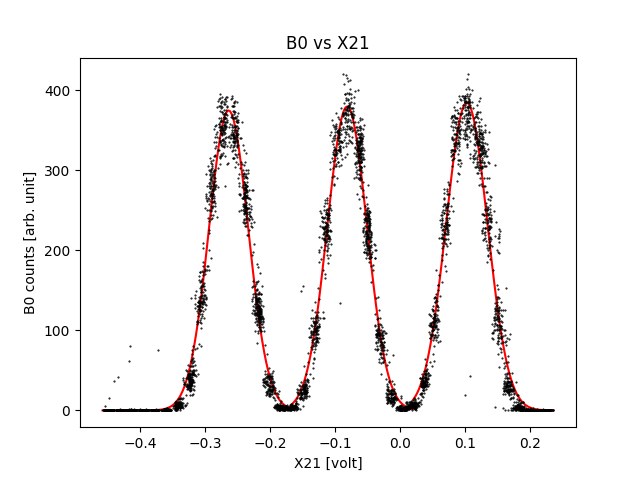
\includegraphics[width=0.7\textwidth]{Analysis/HorizontalCalibration.png}
\caption{•}
\end{figure}

\begin{figure}[hbtp]
\centering
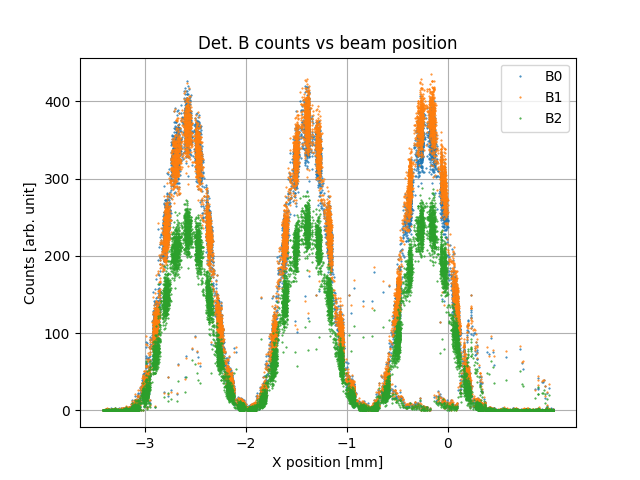
\includegraphics[width=0.45\textwidth]{Analysis/XcheckB.png} 
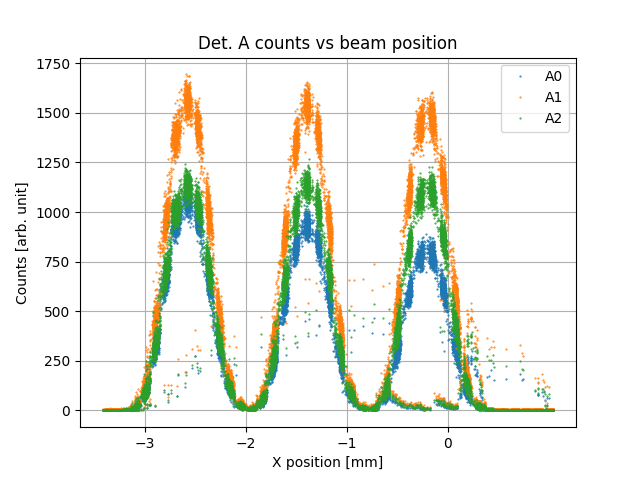
\includegraphics[width=0.45\textwidth]{Analysis/XcheckA.png}
\caption{•}
\end{figure}


\subsection{Current and ENMO monitors}

For the current monitors I13 and I21, we perform the calibration changing the current of the beam and observing the output values of the monitors (Voltage values). The we perform a fit (for the beam current, we used the nominal values that we communicate to MAMI, has the values for the x-axis).

\begin{figure}[hbtp]
\centering
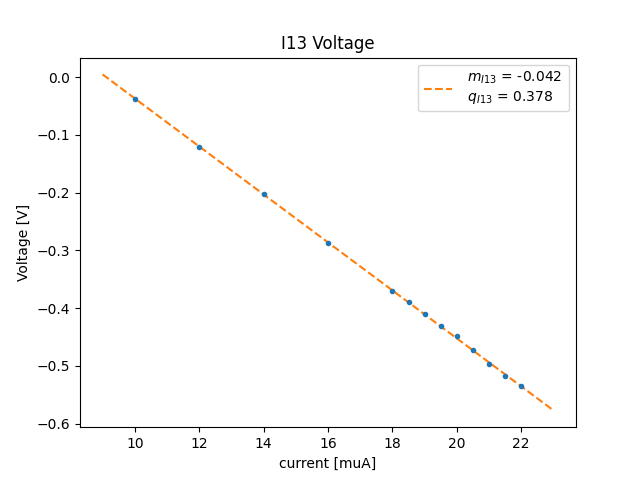
\includegraphics[width = 0.45\textwidth]{Analysis/I13_Calibration.png}
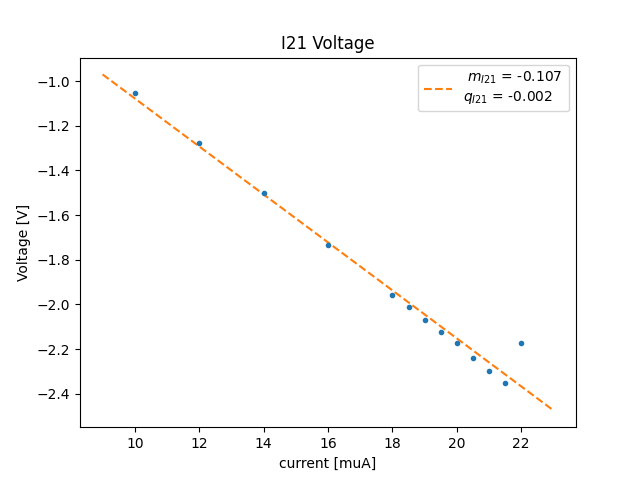
\includegraphics[width = 0.45\textwidth]{Analysis/I21_Calibration.png} 
\caption{•}
\end{figure}

For the two monitors we are able to compute the offset and scale factor:

\begin{equation}
\begin{split}
I^{volt}_{13} = m_{13} \cdot I^{Nom}_{13} + q_{13}\\
c_{13} = \frac{1}{m} \qquad offset = -\frac{q_{13}}{m}
\end{split}
\end{equation}

The same formula for current monitor I21.

The Enmo calibration is performed in a different way from the other monitors. The polarity signal is sent to MAMI, and they produce a signal for the ENMO that somehow (need to investigate exactly how they do that) shows a difference between the first two subevents and the last two. This difference is equal (nominal) to $\SI{22.6}{\kilo \electronvolt}$. The idea now is to produce an histogram for the quantity $\delta E$ (with $E_{18}$ being the energy monitor):

\begin{equation*}
\delta E = \frac{E_{18}[2] + E_{18}[3]}{2} - \frac{E_{18}[0] + E_{18}[1]}{2} 
\end{equation*}

The data should be distributed with a peak around $\SI{22.6}{\kilo \electronvolt}$. To obtain the correct scaling factor for the values stored in the data tree we plot the voltage values mesured by the ENMO monitor.
3 runs of data where taken with different Beam current, to study the dependence of the measured quantity from the beam current. From the mean of the distribution it is possible to exstimate the scaling factor for the ENMO monitors, obtaining the physical quantity in the following way:

\begin{equation*}
C_{E18} = \frac{\SI{22.6}{\kilo \electronvolt}}{\overline{\delta E}}
\end{equation*}

\begin{figure}[hbtp]
\centering
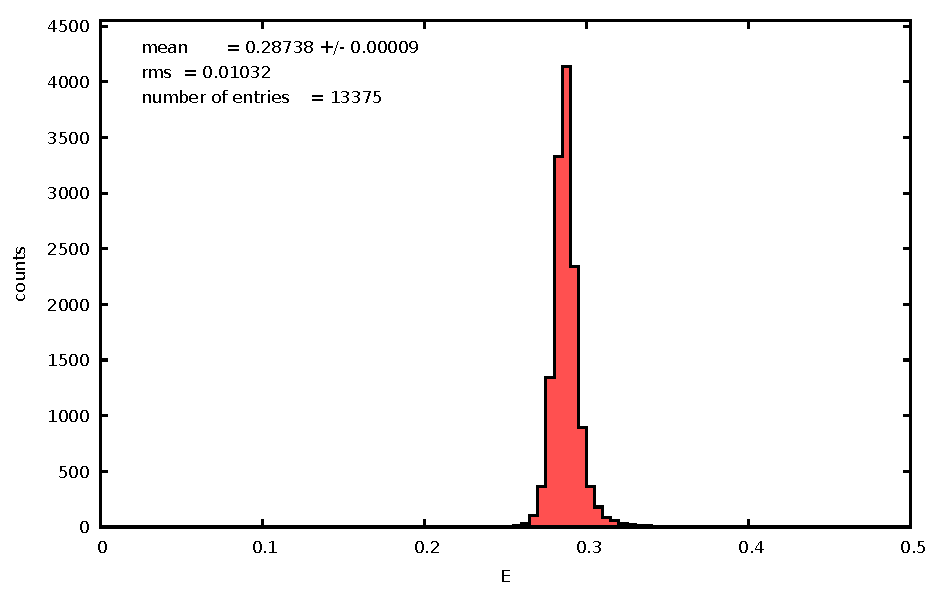
\includegraphics[width = 0.45\textwidth]{Analysis/ENMOvoltage20.pdf}
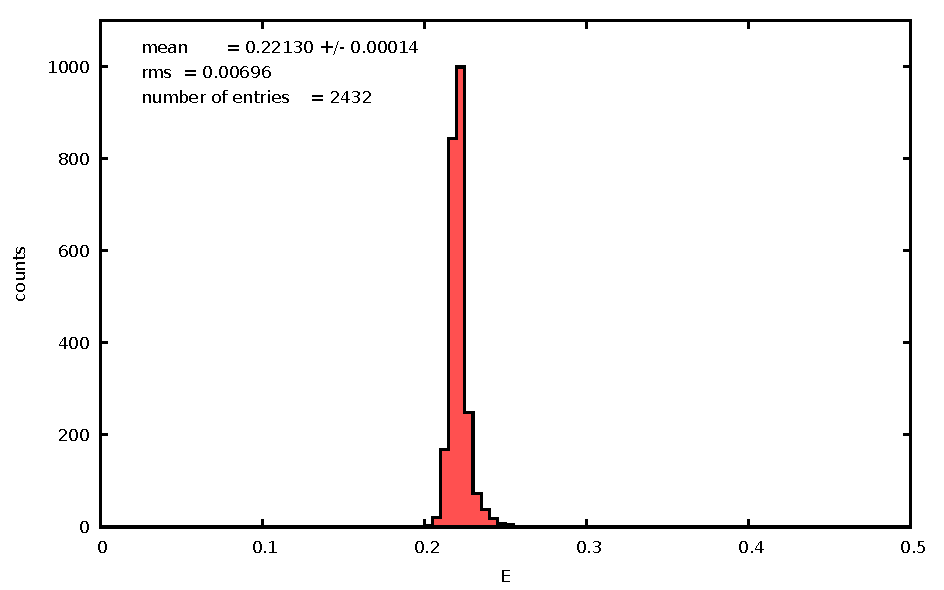
\includegraphics[width = 0.45\textwidth]{Analysis/ENMOvoltage15.pdf} 
\caption{$\delta E$ for 20 $\SI{20}{\micro \ampere}$}
\end{figure}

Taking the average over $E_{18}$ voltage values, and using the formula above, we obtain the coefficient $C_{E18}$. To take care of the current depencende of the monitors, the scaling factor to be placed in the standard.config file is: $C_{E18} \overline{I}_{\mu A}$.
The calibration was performed taking three short acquisitions with different beam current : $\SI{20}{\micro \ampere}$, $\SI{15}{\micro \ampere}$ and a run without beam. 

\begin{figure}[hbtp]
\centering
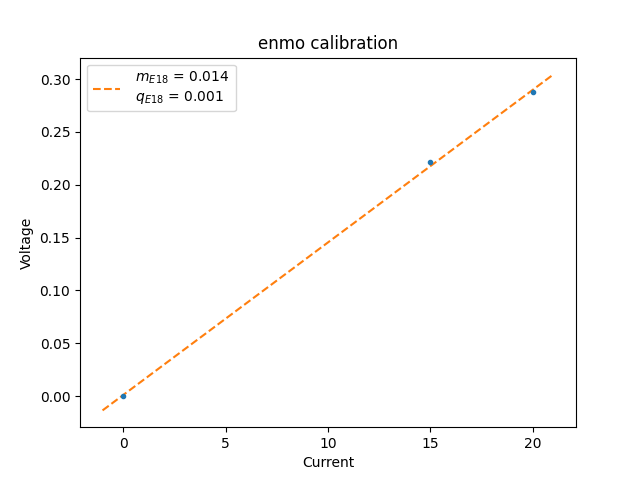
\includegraphics[width = 0.5\textwidth]{Analysis/E18_Calibration.png}
\caption{Calibration of ENMO monitor}
\end{figure}

From this we obtain the value $scaling_{E18} = -1595.2$, to obtain the physical quantity from the analysis. As a final check the final histogram for the physical quantity is shown:

\begin{figure}[hbtp]
\centering
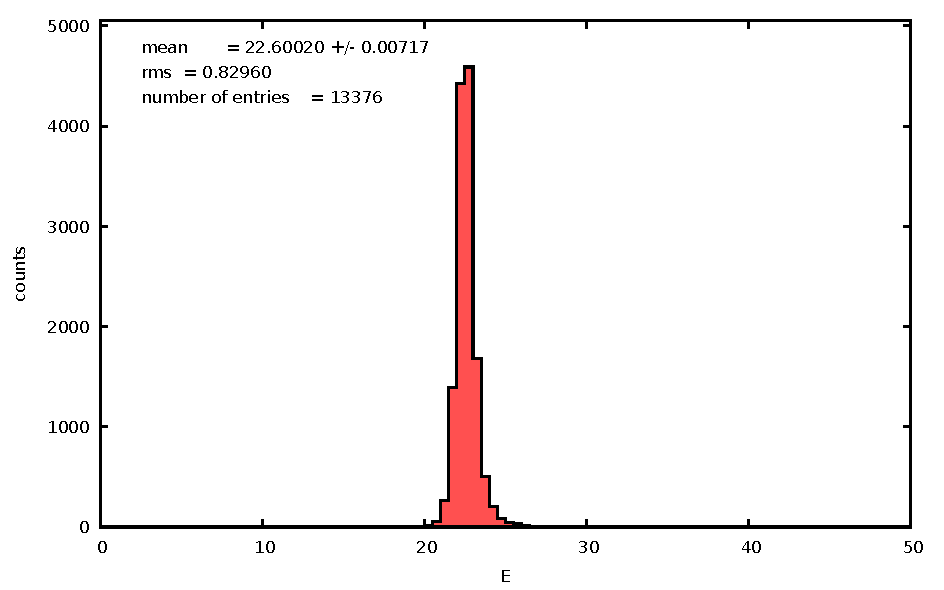
\includegraphics[width = 0.45\textwidth]{Analysis/ENMOCheck20.pdf}
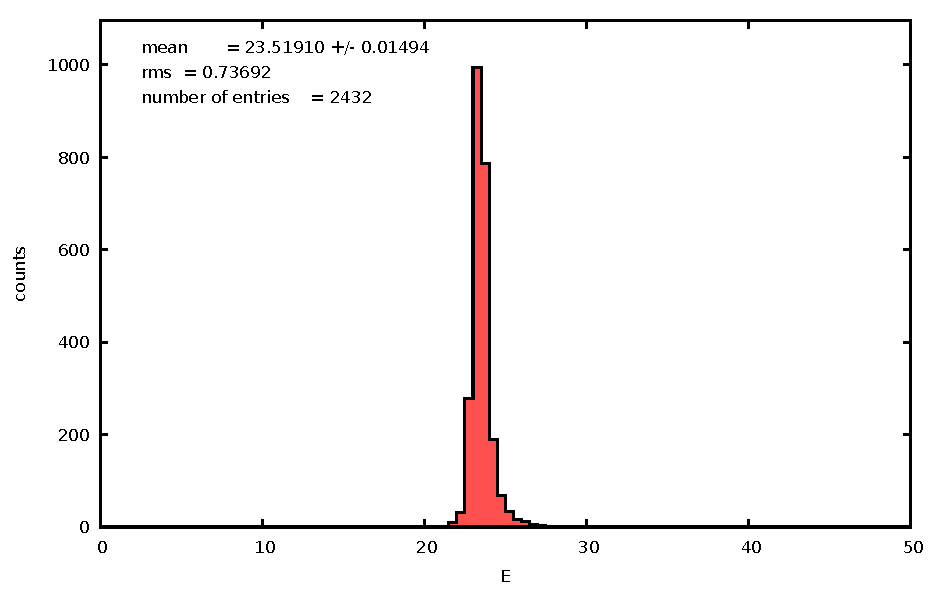
\includegraphics[width = 0.45\textwidth]{Analysis/ENMOCheck15.pdf} 
\caption{Plot for the physical quantities computed in the data tree, for two different current of the beam (on the left $\SI{20}{\micro \ampere}$, $\SI{15}{\micro \ampere}$ on the right)}
\end{figure}

\subsection{Calibration of the pmts}

\texttt{Here it's important to show the plots I made during the beam time. I have to mention the Leo tecniques for the correct interpretation of counts vs attenuation.}\\

During the beam time, several scans in attenuation were performed, before switching MAMI to produce the polarized beam, to choose the best working point for the PMTS of the detectors. The same procedure used in the laboratory was followed, starting from low attenuation and raising up the values. It's possible to get a simple model to describe the particular shape of the following plot taking into account simple assumptions about the type of electrical noise that affect the Nino board, and the \textit{pdf} of the signal produced by the PMTS.\\

The first assumption ("this is not a true assumption, Anselm has a plot of the digitalize charge that proves that") is that accumulated charge collected by the Nino board is well described by a gaussian distribution, the second one is that for small threshold the charge produced by the signals follows a step-function distribution. To explain, let's think that the distribution of the charge collected is of this type (the following figure is just an example, the values ​​do not describe the data collected):

\begin{figure}[hbtp]
\centering
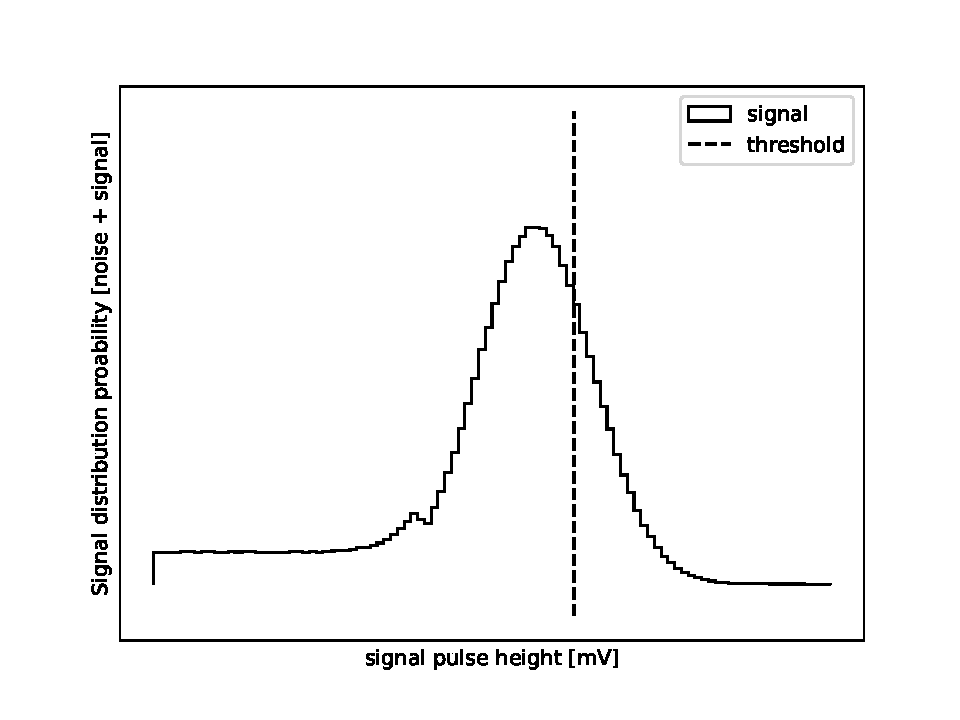
\includegraphics[width = 0.40\textwidth]{Analysis/distribution.pdf}
\caption{Example of the expected distribution of the PMTs output signal}
\end{figure}

The probability for a signal to pass the selection is equal to the probability of being in above the threshold, that is the complementary cumulative of the gaussian distribution (probability of being in the right tail):

\begin{align*}
P(signal > thr) = 1 - \Phi(x) = \dfrac{1 - Erf(\dfrac{x_{thr} - x_{0}}{\sqrt{2} \sigma })}{2}
\end{align*}

Once we reach the uniform zone, the probability of an even being selected is proportional to the area of the rectangle, which increases linearly decreasing the threshold. Considering the normalization factor, it is straightfoward to fit the data with a model of this type:

\begin{equation}
\begin{split}
N(att) = N_{0} \cdot \dfrac{1 + Erf(\dfrac{x_{thr} - x_{0}}{\sqrt{2} \sigma })}{2} \qquad \text{if} \quad att < C  \\
N(att) = N(C) + m \cdot (att - C) \qquad \text{if} \quad att > C
\end{split}
\end{equation}

For the detector B we have the following: 
\begin{figure}[hbtp]
\centering
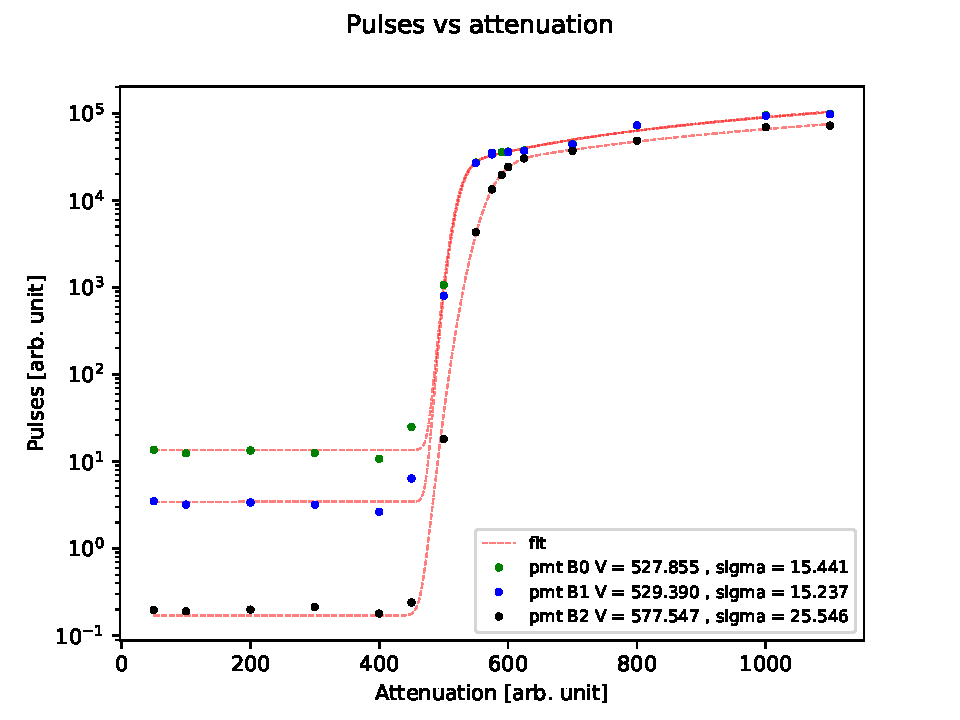
\includegraphics[width = 0.7\textwidth]{Analysis/Fit_attenuation.pdf}
\caption{•}pdf\end{figure}


\subsection{Rates on lead}

This section is straightforward. Basically I have to show the single plot of the pmts counts vs. beam current for lead target. However it's possible to do some preliminary studies, for example to calculate the time needed for measuring the asymmetry on lead with a certain error and maybe check from Mott cross section that the observed rate are fine. 

\begin{figure}[hbtp]
\centering
\includegraphics[width = 0.45\textwidth]{Analysis/Rates_on_lead.png}
\includegraphics[width = 0.45\textwidth]{Analysis/Rates_on_leadB.png}
\caption{Rates on lead Target, for Detector A (left)}
\end{figure}

\section{ $^{12}C$ asymmetry}

\subsection{Autocalibration procedure}

\subsection{least square fit}

When all the calibrations are performed, it is possible to proceed to generate the datafiles fot the fit program. (spiegare in dettaglio come è fatto il programma di analisi)\\
For a better visualization of the data, especially to observe the dependence of the asymmetry on the Beam parameters measured, it is useful to take the average asymmetry at regular intervals. From the raw plots of the asymmetries (see below \ref{fig:asyvsparam}), it is clear that the statistical error associated to the asymmetry is the main one, and it's not possible to identify a linear dependence.

\begin{figure}[hbtp]
\centering
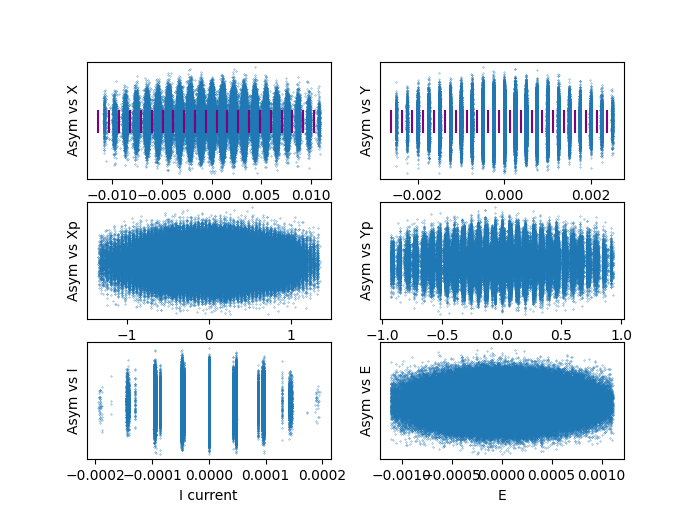
\includegraphics[width = 0.5\textwidth]{Analysis/Asym_vs_monitor.png}
\caption{Asymmetries vs. Beam parameters}
\label{fig:asyvsparam}
\end{figure}

In some plots (X,Y and I) we can identify equally spaced cluster of data. So we decide to compute the averaged asymmetry for each cluster we were able to identify. 
In the following plots we decided to apply some cuts to the data, selecting only the events where the values of all the monitor are less then 3 standard deviation far from the mean. In all the figures the asymmetries are multiplied by a factor of $1e6$ to have the result in ppm (so each y-axis is in ppm). 

\begin{align*}
(x_{monitor} - \overline{x}_{monitor}) \leq 3 \cdot \sigma_{X}
\end{align*}

For each monitor we use the \textit{curve fit} function of the python library \text{scipy} to fit the data. Each Beam parameter is treated separately now, so in principle we are ignoring possible effect of correlation between the X-values (however, from the correlation matrix    \textit{write that somewhere} the effects are negligible)  

\begin{figure}[hbtp]
\centering
\subfloat[][\emph{Asymmetries [ppm] vs X position [$mm$]}]
	{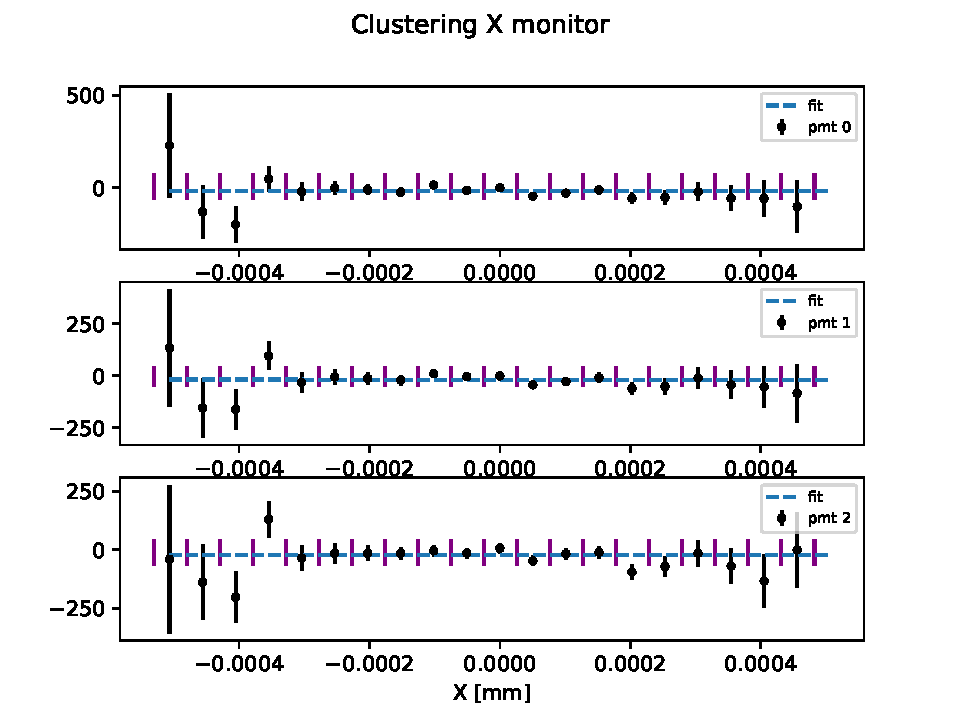
\includegraphics[width = 0.45\textwidth]{Analysis/clustering_XB.pdf}} \quad
\subfloat[][\emph{Asymmetries [ppm] vs Y position[$mm$]}]
	{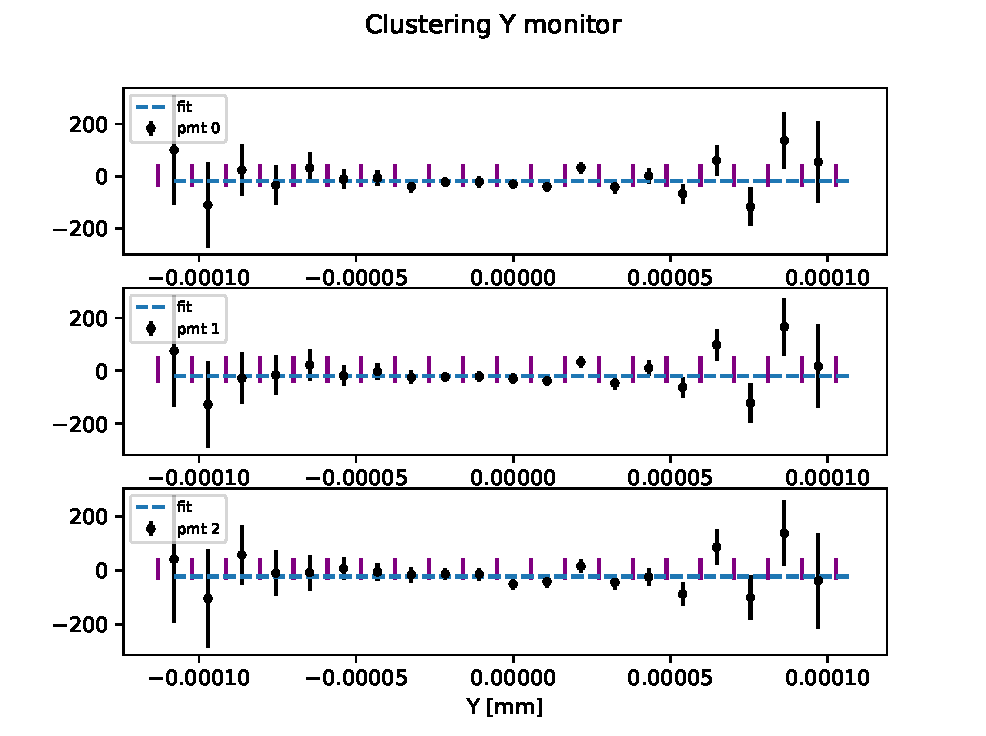
\includegraphics[width = 0.45\textwidth]{Analysis/clustering_YB.pdf}} \\
\subfloat[][\emph{Asymmetries [ppm] vs $\theta_{x}$ angle [$rad$]}]
	{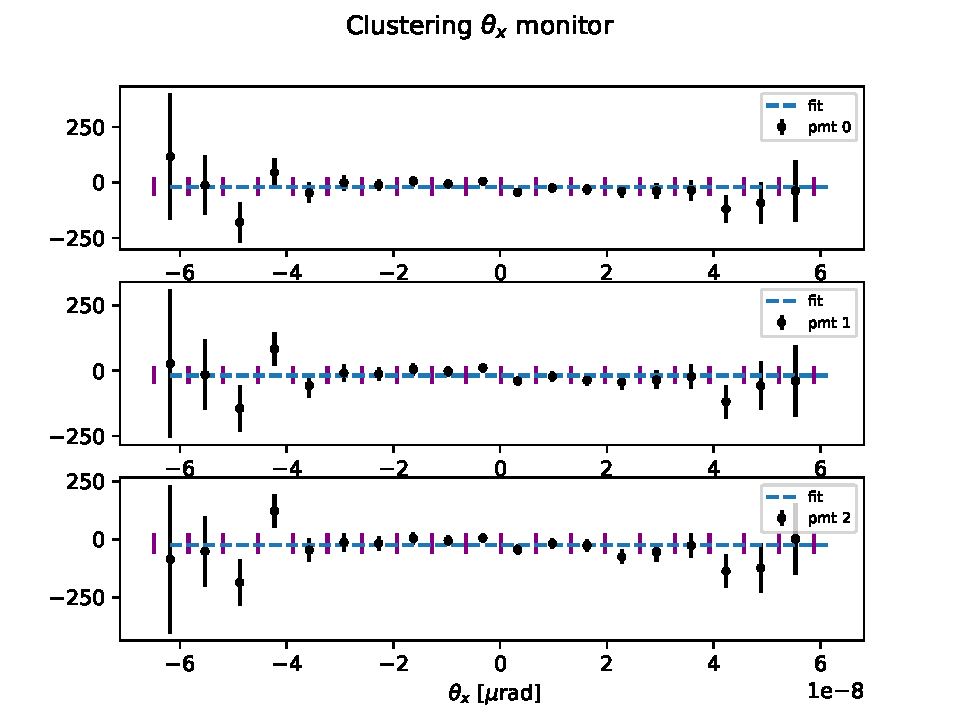
\includegraphics[width = 0.45\textwidth]{Analysis/clustering_XpB.pdf}} \quad
\subfloat[][\emph{Asymmetries [ppm] vs $\theta_{y}$ angle [$rad$]}]
	{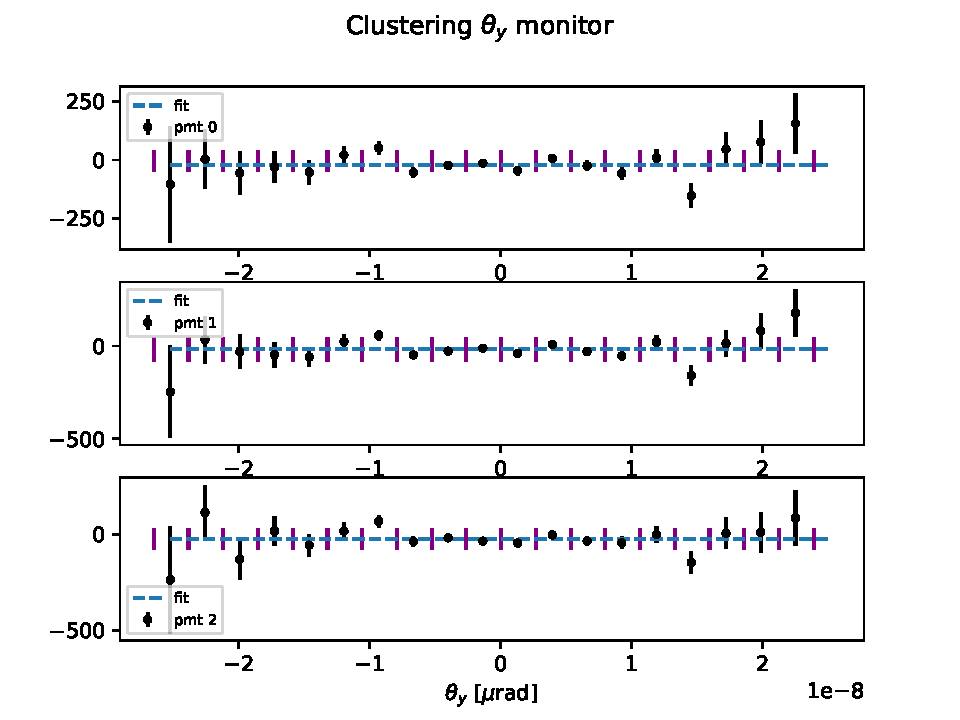
\includegraphics[width = 0.45\textwidth]{Analysis/clustering_YpB.pdf}} \\
\subfloat[][\emph{Asymmetries [ppm] vs E [$keV$]}]
	{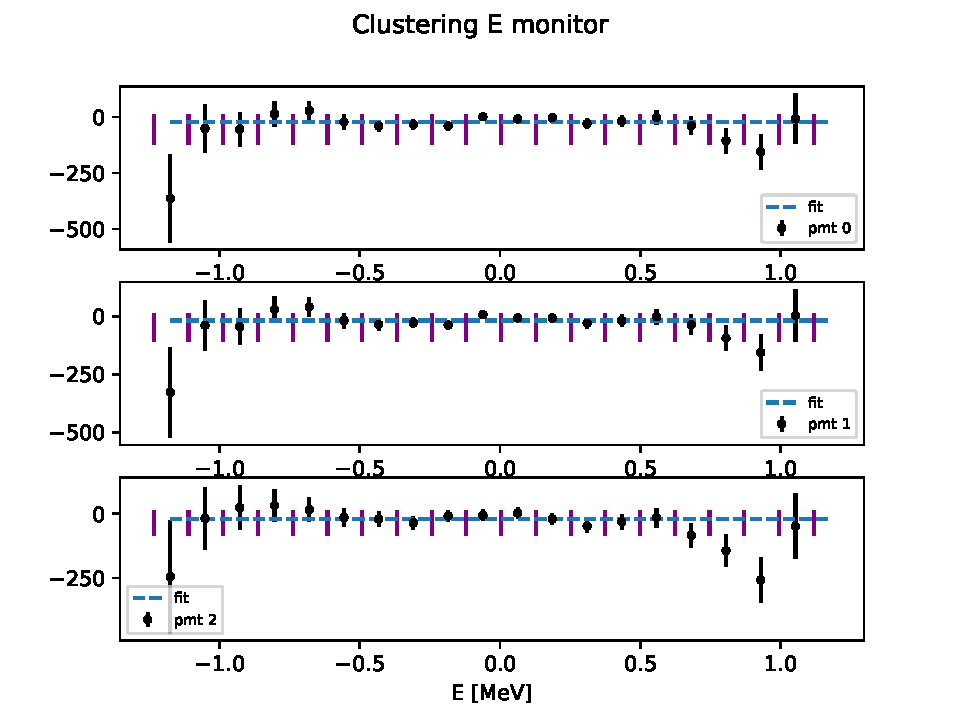
\includegraphics[width = 0.45\textwidth]{Analysis/clustering_EB.pdf}} \quad
\subfloat[][\emph{Asymmetries [ppm] vs I current [arb.unit]}]
	{\includegraphics[width = 0.45\textwidth]{Analysis/clustering_IB.pdf}} \quad
\label{fig:averageAsym}
\end{figure}

\begin{figure}[hbtp]
\centering
\subfloat[][\emph{Asymmetries [ppm] vs X position [$mm$]}]
	{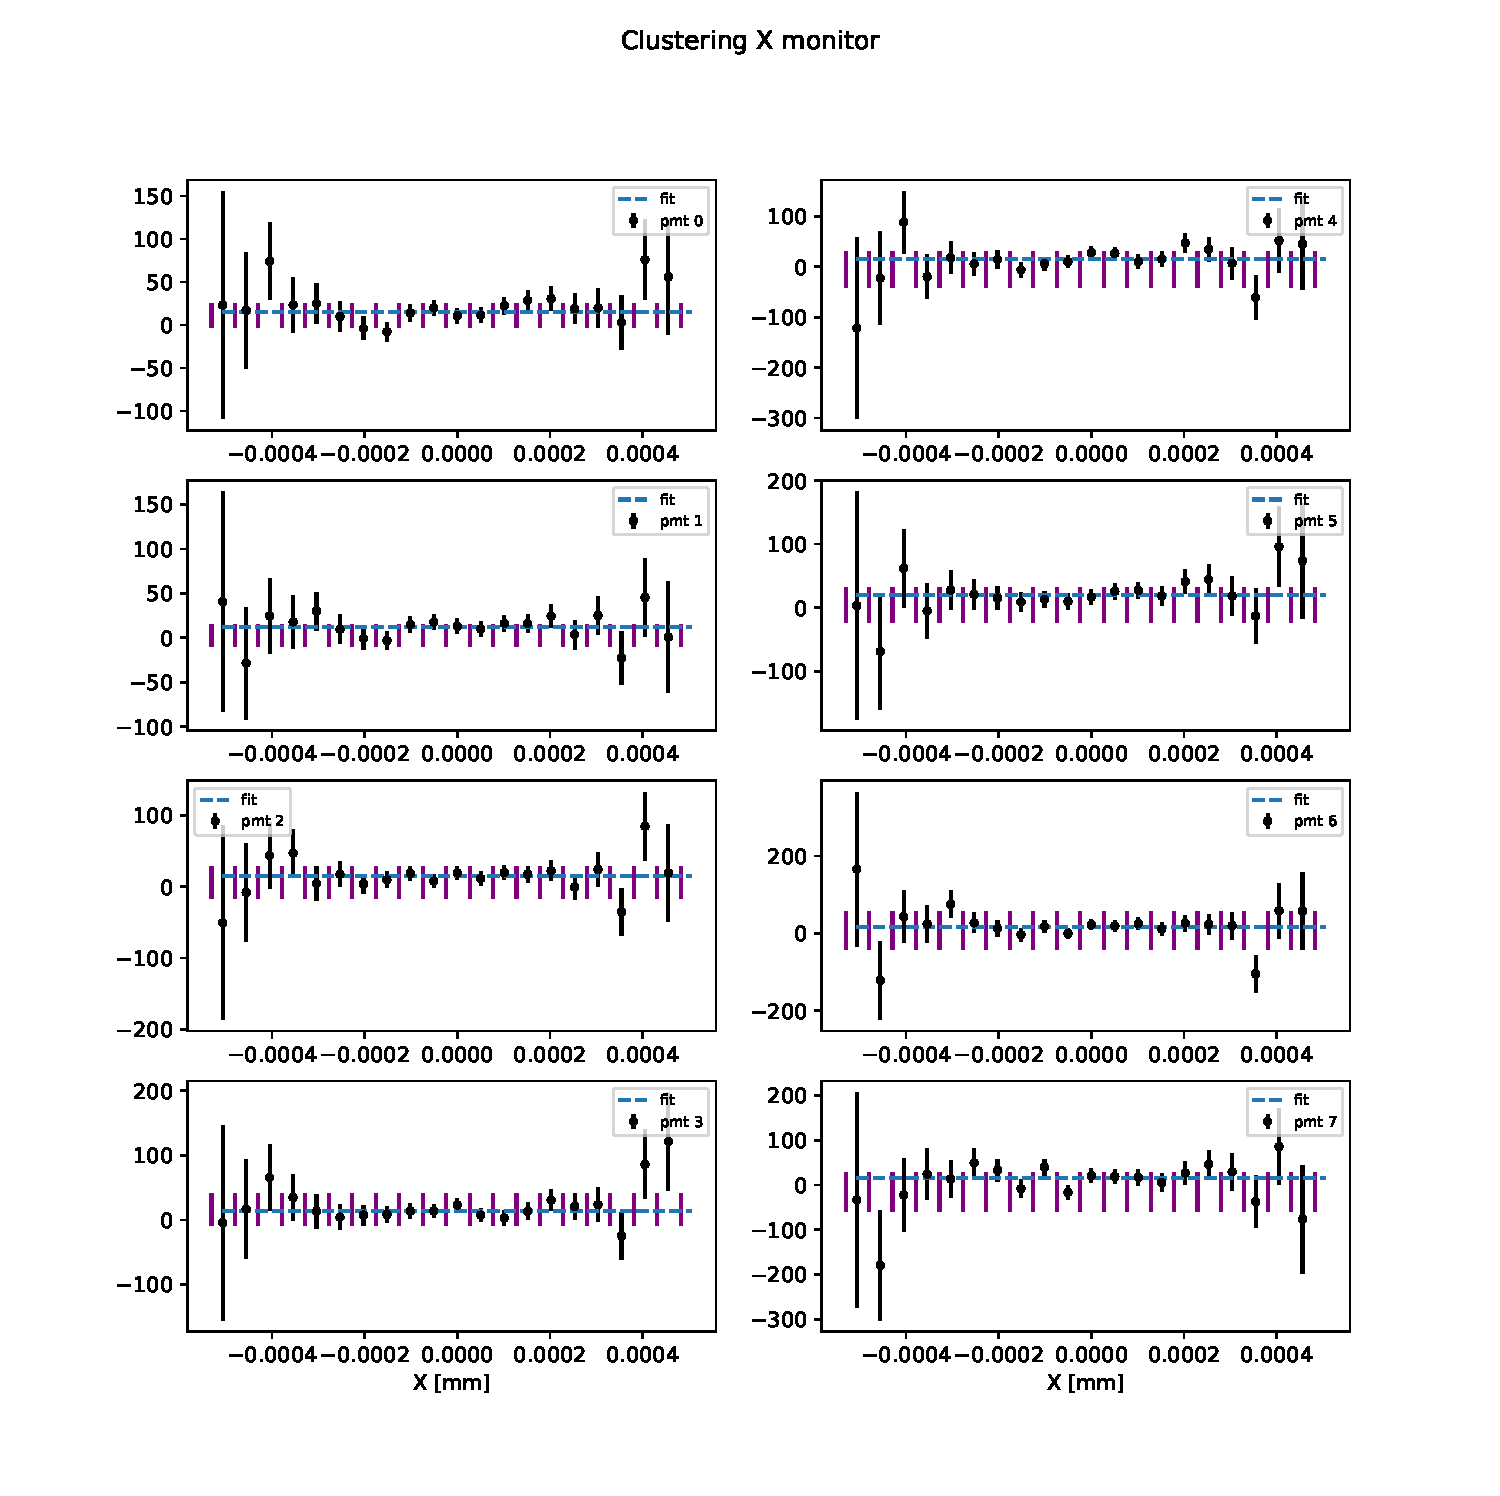
\includegraphics[width = 0.45\textwidth]{Analysis/clustering_XA.pdf}} \quad
\subfloat[][\emph{Asymmetries [ppm] vs Y position[$mm$]}]
	{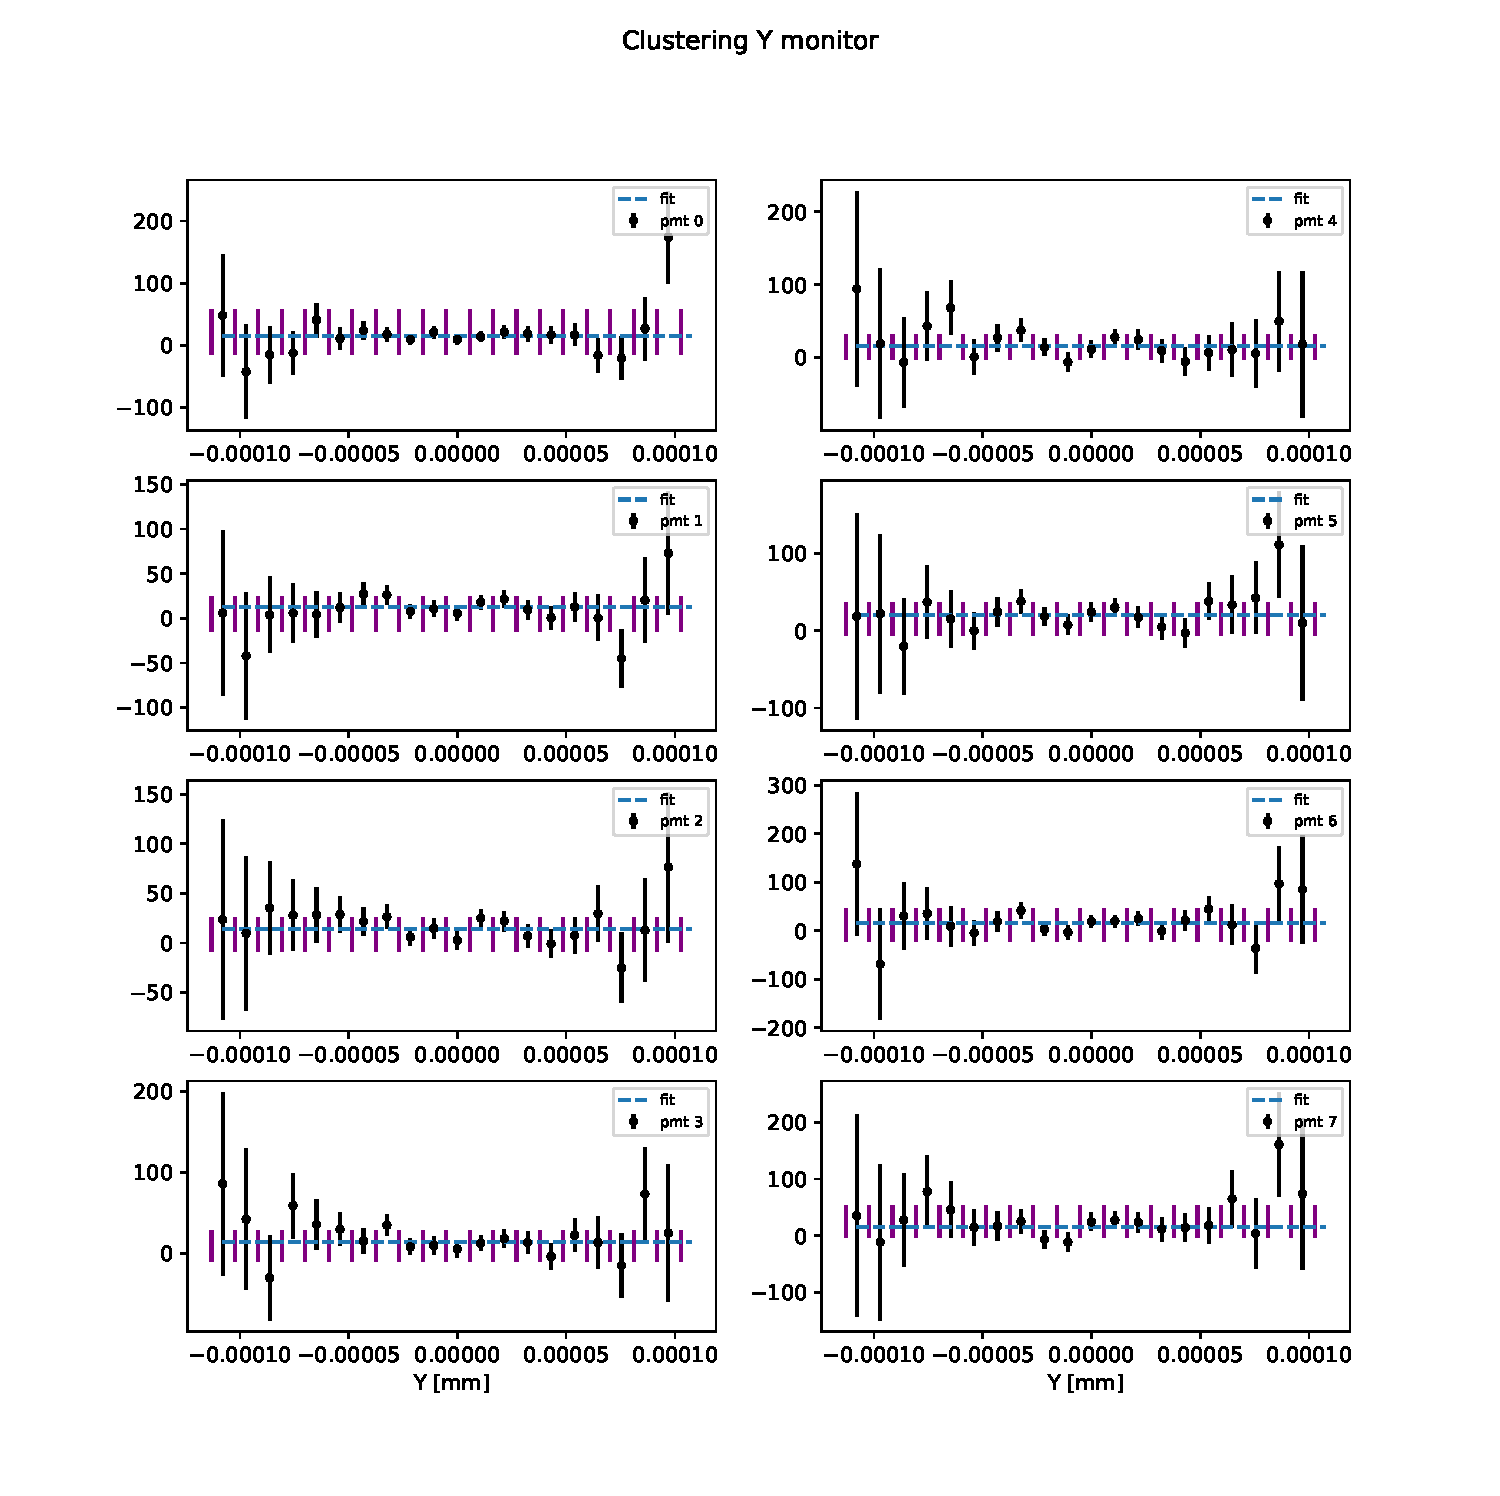
\includegraphics[width = 0.45\textwidth]{Analysis/clustering_YA.pdf}} \\
\subfloat[][\emph{Asymmetries [ppm] vs $\theta_{x}$ angle [$rad$]}]
	{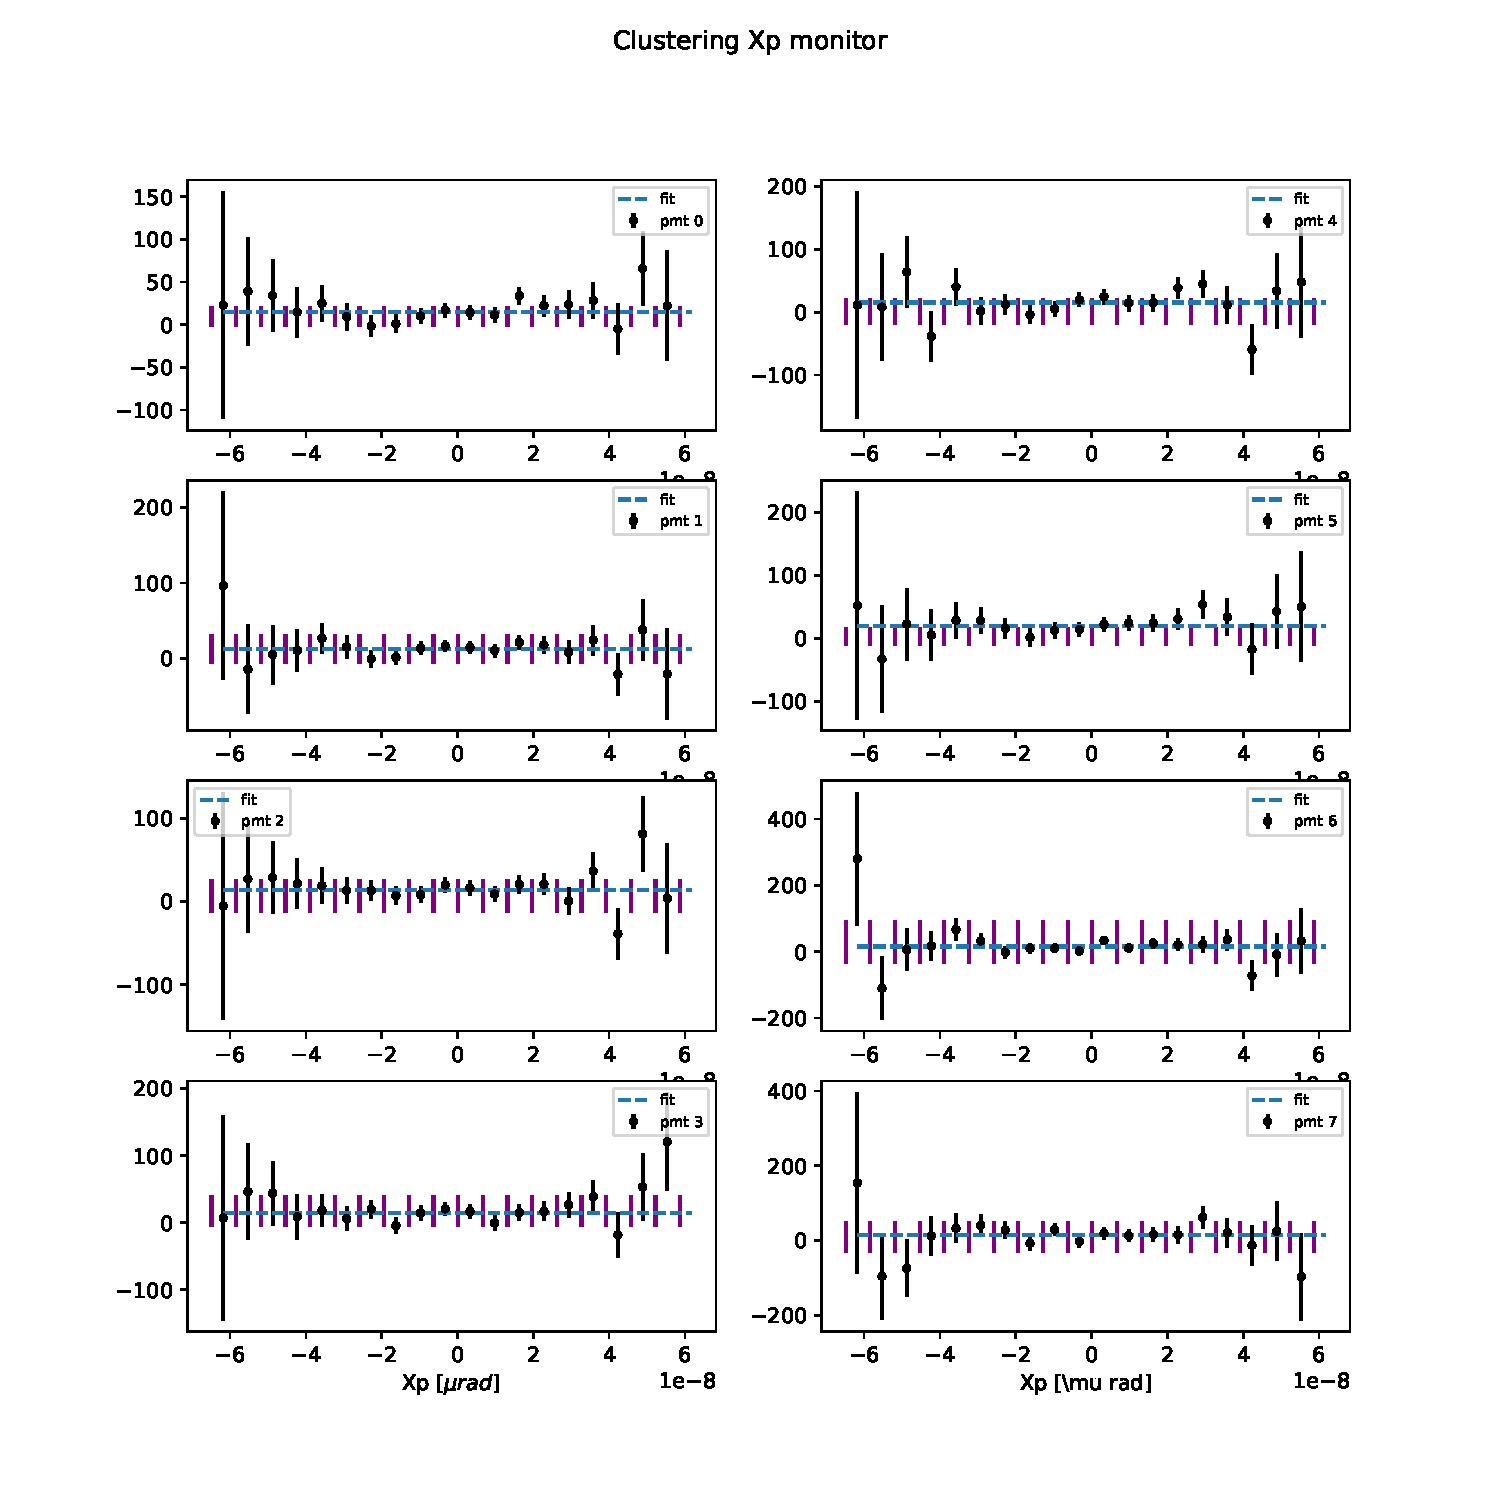
\includegraphics[width = 0.45\textwidth]{Analysis/clustering_XpA.pdf}} \quad
%\subfloat[][\emph{Asymmetries [ppm] vs $\theta_{y}$ angle [$rad$]}]
%	{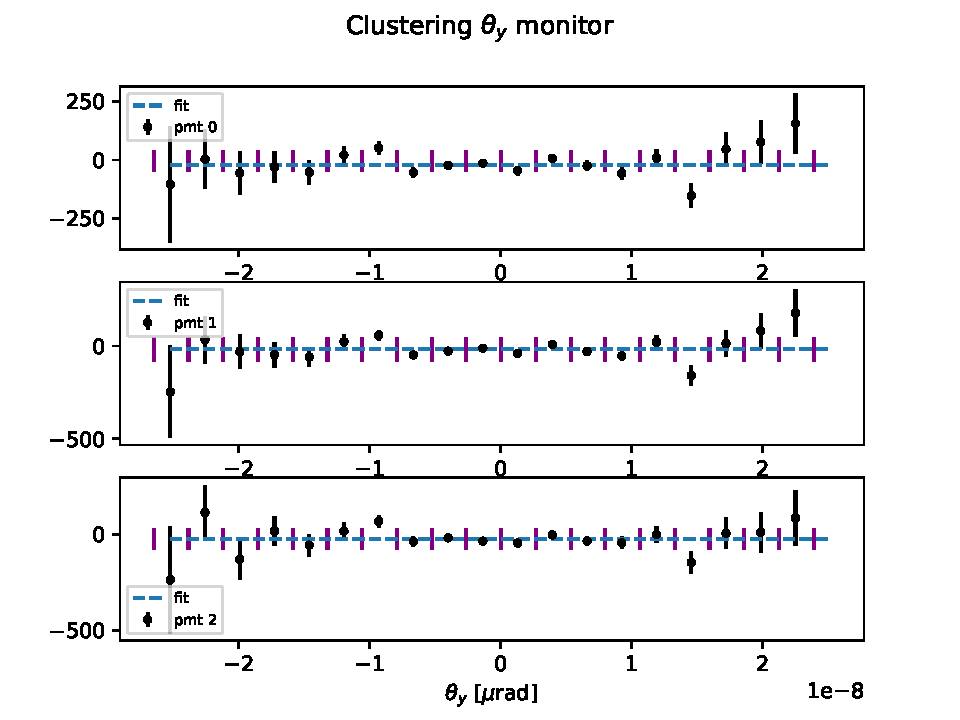
\includegraphics[width = 0.45\textwidth]{Analysis/clustering_YpB.pdf}} \\
%\subfloat[][\emph{Asymmetries [ppm] vs E [$keV$]}]
%	{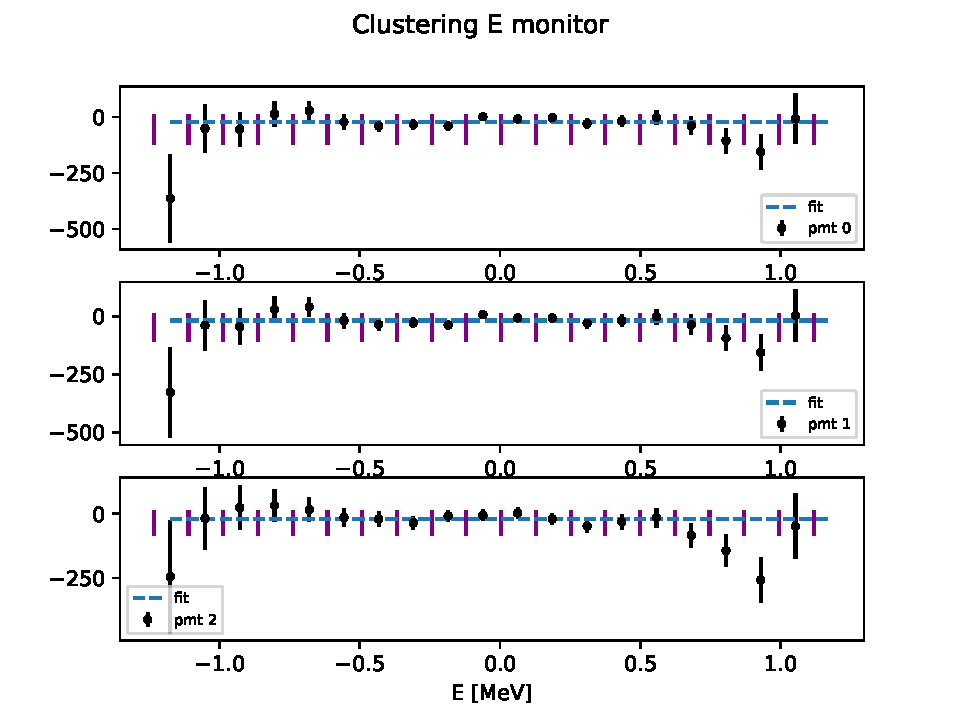
\includegraphics[width = 0.45\textwidth]{Analysis/clustering_EB.pdf}} \quad
%\subfloat[][\emph{Asymmetries [ppm] vs I current [arb.unit]}]
%	{\includegraphics[width = 0.45\textwidth]{Analysis/clustering_IB.pdf}} \quad
\label{fig:averageAsym}
\end{figure}


The error of each point is computed exploiting the same formula defined above (theory section; $N_{A/B}$ averaged pmt counts for each subevents and $n$ number of event in each interval):

\begin{align*}
\sigma_{Asym} = \dfrac{1}{\sqrt{2N_{A/B} \cdot n}}
\end{align*}

From this plots we can check if the linear model is good enough to descrive the depencence of out data and decide if the it should be useful to apply different cuts for certain beam parameters. We report now a first exstimation of the false asimmetries, later the data will be fitted without treat separately the beam parameters. From that we can learn the effects of the correlation between the data.

\begin{center}
\begin{tabular}{||c|c|c|c|c|}
\hline
pmt: & B0 & B1 & B2 & unit \\ 
\hline 
$\frac{dA}{dX} $  & $-66 \pm 37$ & $-65 \pm 37$ & $-80 \pm 47$ & $ \frac{ppm}{\SI{}{\micro \meter}}$\\ 
\hline 
$\frac{dA}{dY} $  & $34 \pm 219$  & $ 79 \pm 233$ & $ -213 \pm 219$ & $\frac{ppm}{\SI{}{\micro \meter} }$ \\ 
\hline 
$\frac{dA}{d\theta_{y}}$ & $-416 \pm 1181$  & $ -443 \pm 1227$ & $-1237 \pm 1130$ & $\frac{ppm}{\mu rad}$\\ 
\hline 
$\frac{dA}{d\theta_{x}}$ & $-672 \pm 297$ & $ -672 \pm 307 $ & $-845 \pm 380$ & $\frac{ppm}{\mu rad}$ \\ 
\hline 
$\frac{dA}{dE}$ & $ -0.004 \pm 0.016 $ & $-0.011 \pm 0.016 $ & $ - 0.044 \pm 0.018 $ & $\frac{ppm}{\SI{}{\kilo \electronvolt}}$\\ 
\hline
\end{tabular} 
\end{center}


\subsection{False asymmetries}
Seems that is possible to obtain rough estimates of the beam related asymmetries with the results from the fit. For Energy and position it's achievable, while for the angles it's quite hard (in principle sounds possible to perform an analytic calculation of the asymmetry related to the incident beam angle, however Anselm told me that quite often those results are in disagrement with the observed even in the sign!).  

\subsection{??Bootstrap??}

Although Anselm was against it, now seems possible to increase the precision of the mesurement with a procedure similar to a bootstrap. Instead of computing all the quantities inside a single event, it's possible to compute all the important quantities also between different events. In this scenario the statistics can be increased artificially as mutch as we want, with the same amount of data. Of course, it's also simple to abuse of this method, so we should restrict using only events next to each other. However seem reasonable and promising.

\subsection{??interval estimation??}




